\section{Results Overview}

\subsection{Real Data}
\begin{figure}[htp]
	\centering
	\begin{subfigure}{0.3\textwidth}
		\centering
		\begin{lstlisting}[language=R,basicstyle=\tiny]
		
Levin-Lin-Chu Test
Stationary:     27
Non-stationary: 8

		\end{lstlisting}
	\end{subfigure}
\begin{subfigure}{0.3\textwidth}
	\centering
	\begin{lstlisting}[language=R,basicstyle=\tiny]

Maddala-Wu Test
Stationary:     7
Non-stationary: 28

	\end{lstlisting}
\end{subfigure}
\begin{subfigure}{0.3\textwidth}
	\centering
	\begin{lstlisting}[language=R,basicstyle=\tiny]

IPS Test
Stationary:     22
Non-stationary: 13

	\end{lstlisting}
\end{subfigure}

\caption{Summary of Panel Test results.}
\end{figure}


The results in Figure 5.1 clearly show that the Levin-Lin-Chu test strongly rejects the null hypothesis of the data following a unit root majority of the time. There are a few cases where the tests results indicate that the panels are not stationary, but these are instances where the panel dimensions are $N \to 0$ and $T \to \inf$. The IPS test results indicate stationarity in the panels as a whole, but a larger minority of non-stationary results was present here than in the Levin-Lin-Chu or Maddala-Wu. By contrast, the individual tests (results shown in Figure 2), the Augmented Dickey Fuller and Phillips-Perron, both overwhelmingly state that most of the time series they test are not stationary. An interesting characteristic of the data is that the test statistic of the individual unit root tests changed by a relatively large degree when single observations were removed, which suggests that the tests were not robust to small sample sizes.

\begin{figure}[htp]
	\centering
	\begin{lstlisting}[language=R]
	===============
	Summary Results
	===============
	ADF Test
	Stationary: 2   Non-Stationary: 34
	PP Test
	Stationary: 0   Non-Stationary: 36
	\end{lstlisting}
	\caption{Results of individual tests}
\end{figure}



\subsection{Simulated Data}

The results of the simulations were re-arranged into graphs where the x-axis was the time dimension, increasing to the right, the y-axis was the individual dimension, ascending, and the colours correspond to the average p-value generated, with green being at or below 0.01, yellow is 0.05 and red is 0.1 and above.

\begin{figure}[htp]
	\centering
	\begin{subfigure}{0.3\textwidth}
		\centering
		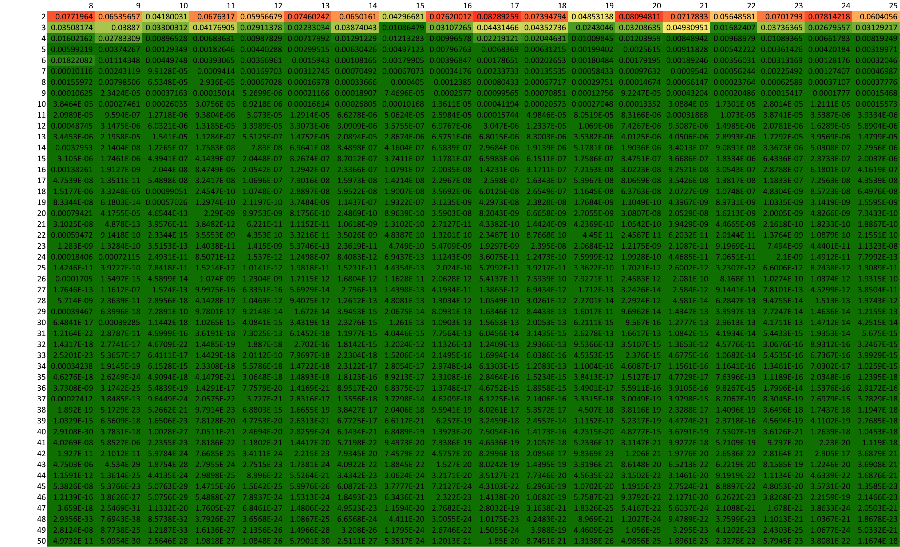
\includegraphics[width= \linewidth]{llc-050}
	\end{subfigure}
	\begin{subfigure}{0.3\textwidth}
	\centering
	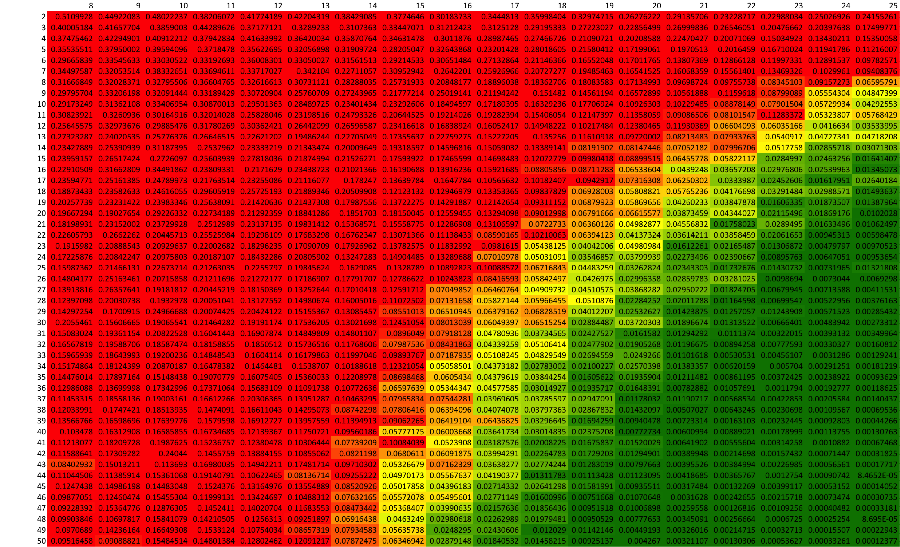
\includegraphics[width= \linewidth]{mw-050}
\end{subfigure}
	\begin{subfigure}{0.3\textwidth}
	\centering
	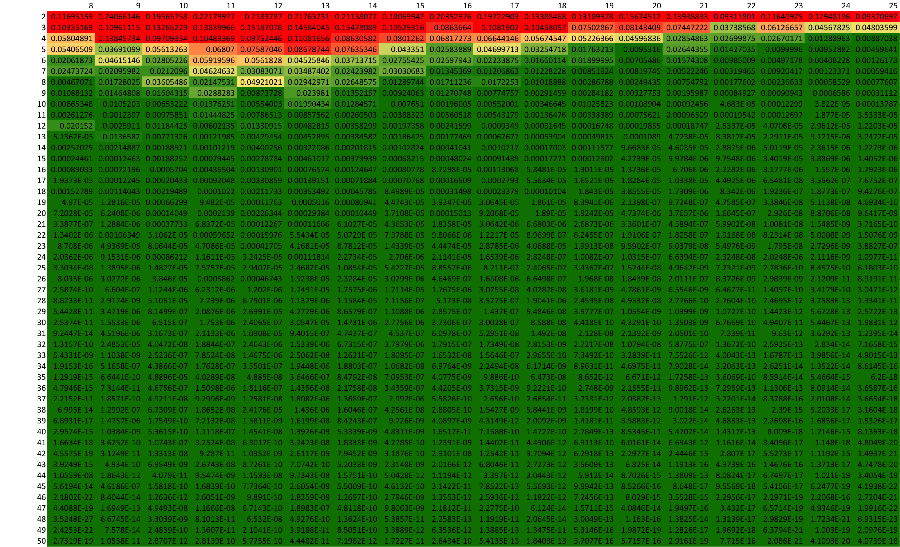
\includegraphics[width= \linewidth]{ips-050}
\end{subfigure}
\caption{Results for the Levin-Lin-Chi, Maddala-Wu and IPS when $\rho = 0.5$ (from left to right)}
%\subcaption{Note: the x-axis is T and the y-axis is N}
\end{figure}
%Note: In this section, I would include heat-maps with the 

The simulations initially seemed to show the Maddala-Wu performing better than the Levin-Lin-Chu when it came to correctly identifying datasets with $\rho$ less than but very close to 1, meaning they were on the verge of having a unit root. However, this was discovered to be due to the programming error discussed in Chapter 4, and the real results for the Maddala-Wu showed an overwhelming tendancy to fail to reject the null hypothesis. The IPS, on the other hand, appeared to perform comparably to the Levin-Lin-Chu at $\rho = 0.5$. When compared to the Levin-Lin-Chu, the Maddala-Wu was quicker to move away from rejection territory as $\rho \to 1$, but the IPS moved further from rejection territory as the $T \to \infty$. With that said,both the Levin-Lin-Chu and IPS seemed be accurate at rejecting the null when $\rho = 0.5$.

\begin{figure}[htp]
	\centering
	\begin{subfigure}{0.3\textwidth}
		\centering
		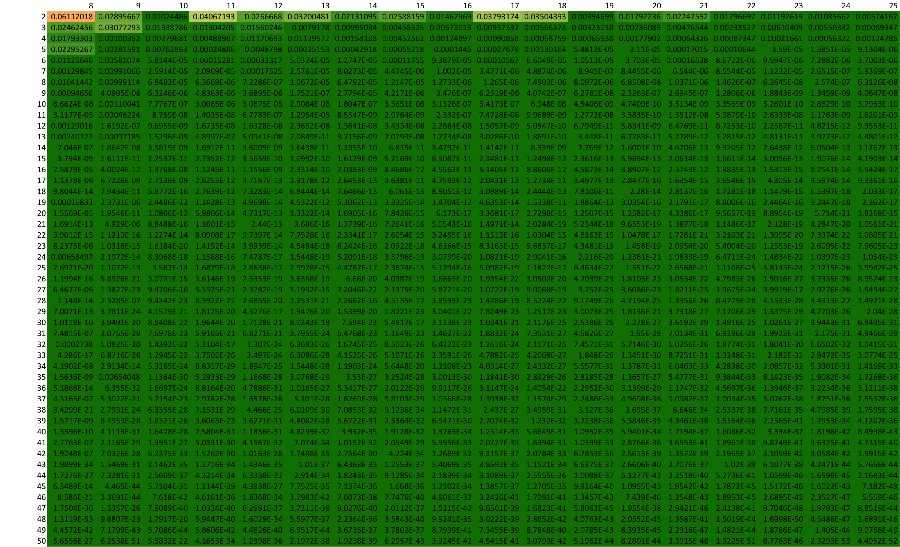
\includegraphics[width= \linewidth]{llc-075}
	\end{subfigure}
	\begin{subfigure}{0.3\textwidth}
		\centering
		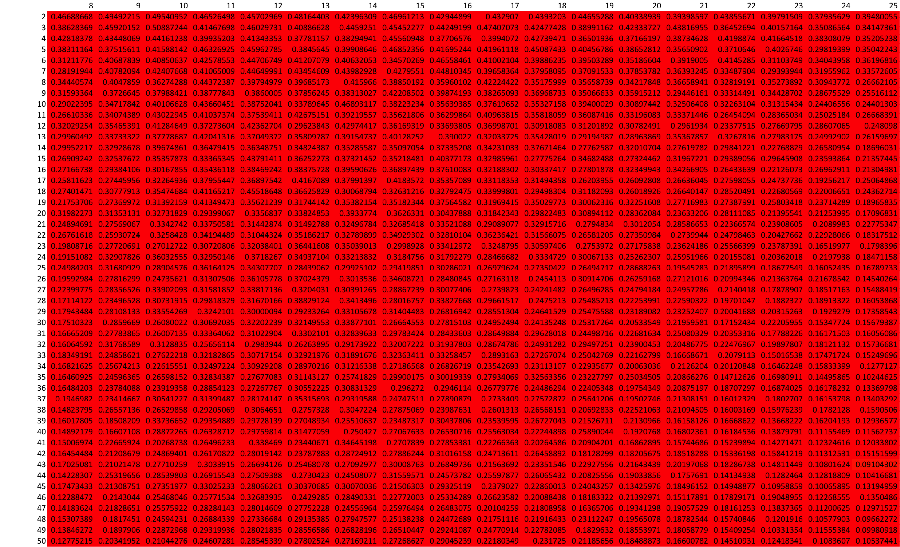
\includegraphics[width= \linewidth]{mw-075}
	\end{subfigure}
	\begin{subfigure}{0.3\textwidth}
		\centering
		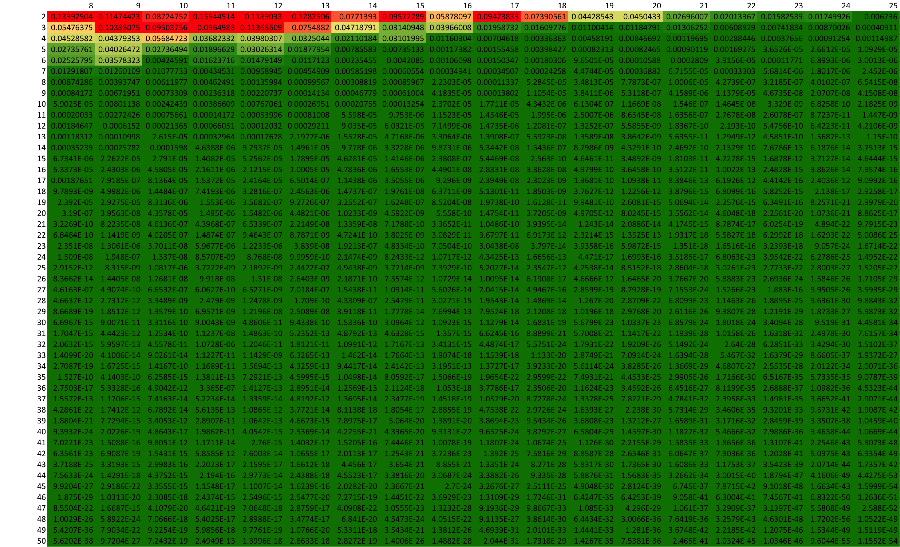
\includegraphics[width= \linewidth]{ips-075}
	\end{subfigure}
	\caption{Results for the Levin-Lin-Chi, Maddala-Wu and IPS when $\rho = 0.75$ (from left to right)}
	%\subcaption{Note: the x-axis is T and the y-axis is N}
\end{figure}

Moving to the case of $\rho = 0.75$, the Levin-Lin-Chu and IPS performed nearly identically with regards to rejecting the null and panel dimensions as with the previous case. The Maddala-Wu, on the other hand, wholly failed to reject the null on average for all panel dimensions tests for $\rho = 0.75$ as well as $\rho = 0.9$ and $\rho = 1$.

\begin{figure}[htp]
	\centering
	\begin{subfigure}{0.3\textwidth}
		\centering
		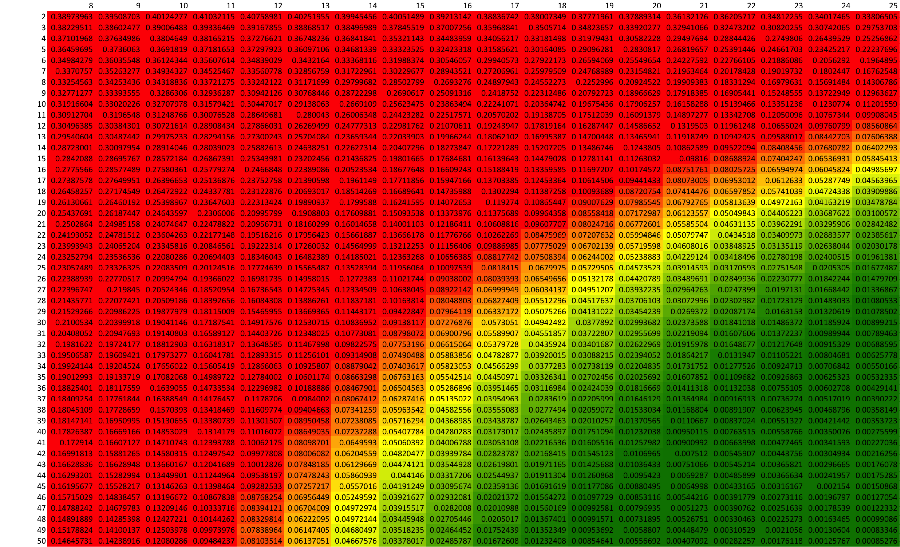
\includegraphics[width= \linewidth]{llc-090}
	\end{subfigure}
	\begin{subfigure}{0.3\textwidth}
		\centering
		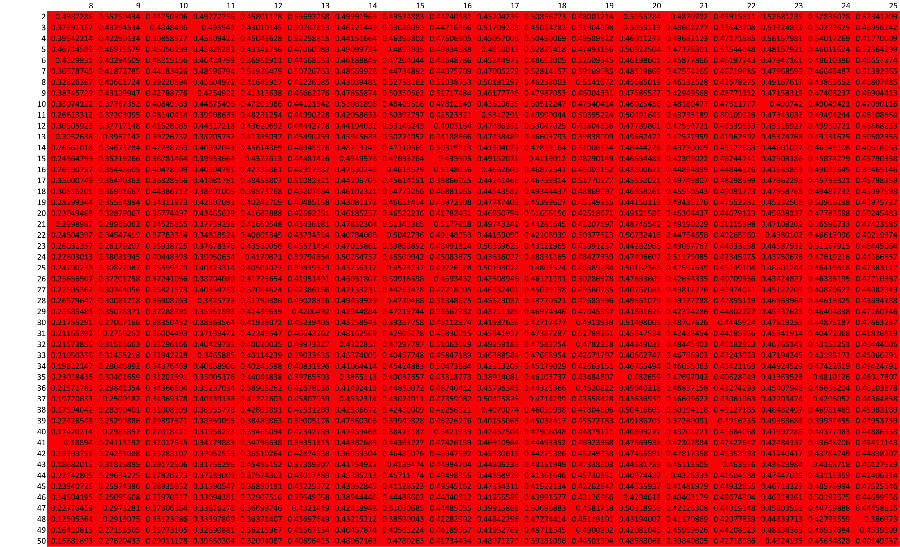
\includegraphics[width= \linewidth]{mw-090}
	\end{subfigure}
	\begin{subfigure}{0.3\textwidth}
		\centering
		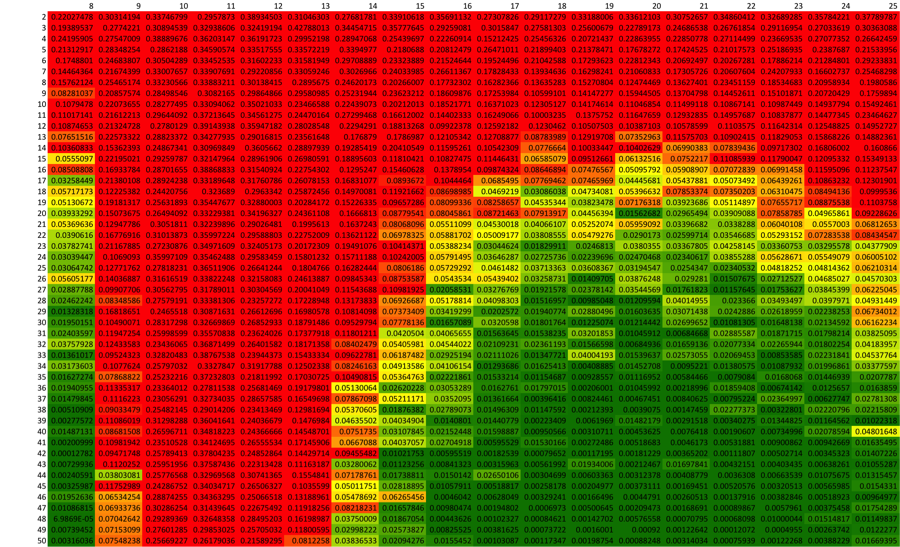
\includegraphics[width= \linewidth]{ips-090}
	\end{subfigure}
	\caption{Results for the Levin-Lin-Chi, Maddala-Wu and IPS when $\rho = 0.9$ (from left to right)}
	%\subcaption{Note: the x-axis is T and the y-axis is N}
\end{figure}


The case of $\rho = 0.9$ began to show more of the relationship between the panel dimensions and null rejection. The Levin-Lin-Chu demonstrated that as $N$ and $T \to \infty$, the power of the test increases and it moves away from Type I errors, where the null hypothesis is wrongly not rejected. The Maddala-Wu, as stated previously, continued to demonstrate complete failure to reject the null hypothesis. The Im-Persaran-Shin test began to exhibit an odd trait, however, as there appeared to not be as clear a relationship between panel dimensions and p-values, at least not a linear one. This curiosity continued in the subsequent test, albeit to a lesser degree.

\begin{figure}[htp]
	\centering
	\begin{subfigure}{0.3\textwidth}
		\centering
		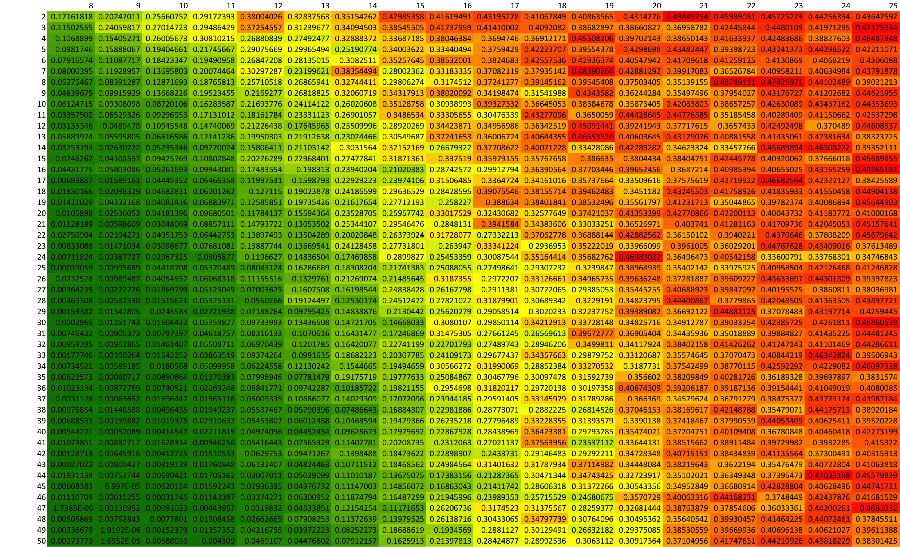
\includegraphics[width= \linewidth]{llc-100}
	\end{subfigure}
	\begin{subfigure}{0.3\textwidth}
		\centering
		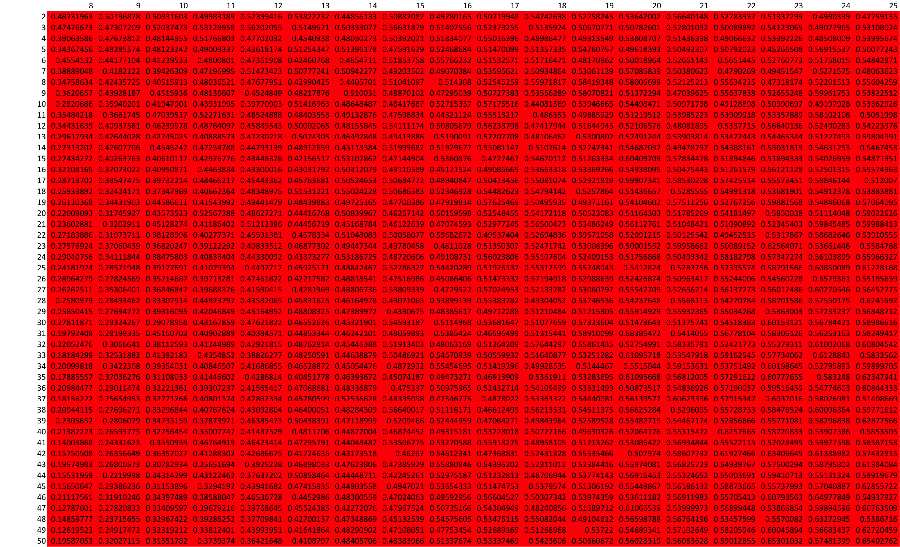
\includegraphics[width= \linewidth]{mw-100}
	\end{subfigure}
	\begin{subfigure}{0.3\textwidth}
		\centering
		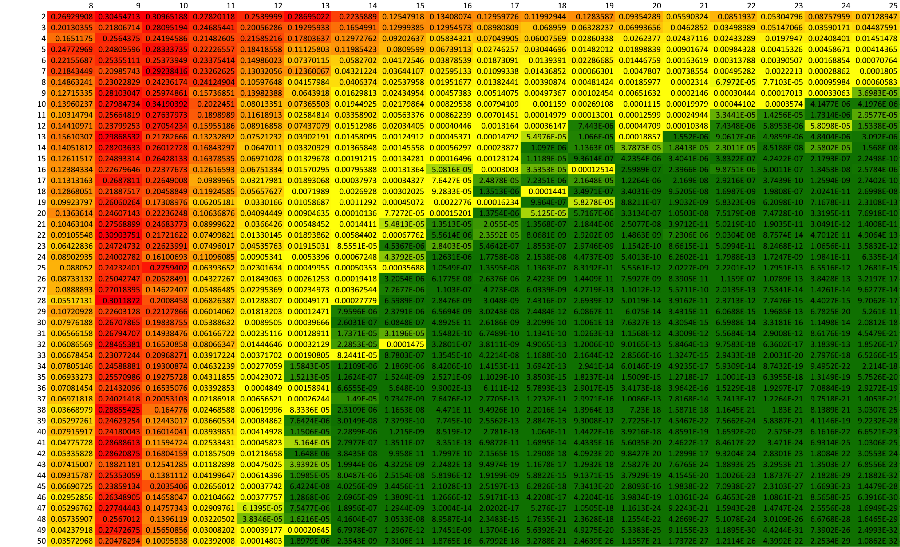
\includegraphics[width= \linewidth]{ips-100}
	\end{subfigure}
	\caption{Results for the Levin-Lin-Chi, Maddala-Wu and IPS when $\rho = 1$ (from left to right)}
	%\subcaption{Note: the x-axis is T and the y-axis is N}
\end{figure}

The final case which was examined was the case of a unit root, or where $\rho = 1$. The most notable result here was the Levin-Lin-Chu test, which appeared to reverse its relationship with the dimensions of the panel. As the panel increased in size, the Levin-Lin-Chu test was less likely to reject the null hypothesis of a unit root. The Maddala-Wu performed identically to the way it had in the previous cases. The Im-Persaran-Shin, however, began to have a more linear relationship with the dimensions of the panel, albeit with the small tendency to reject the null for cases where $N$ was high but $T$ was low.

\section{Analysis}

\subsection{Real Data}

The panel unit root tests done on the real data overwhelmingly rejected the null hypothesis of a unit root (with the exception of the Maddala-Wu), while the time series tests very quickly began to fail to reject the null hypothesis of a unit root as the time series dimension fell. The key question with the real data is whether the results are spurious or have actual value. As noted above, the individual tests did not show consistency, significantly changing the critical value from rejection territory to non-rejection territory with only one observation removed and vice versa. This exemplifies the criticism often levied at single time series stationarity tests, in that for time series with a small number of observations (below 100), the tests have extremely limited power, meaning that even if the single stationarity test indicated a time series was correctly stationary, the result was most likely spurious and coincidental. It is important to note how the panel unit root tests behaved when the time series dimension was large but the individual dimension was low. The panel tests tended to show that the panels were not stationary, but it is important to view these results in light of the Monte Carlo simulations. In the MC simulations, it was shown that the tests quickly converge to a p-value as individual dimensions are added, while the initial p-value is quite high for an individual dimension of 2 or 3 (therefore failing to reject the null of a unit root). It therefore follows that the tests have a power similar to that of single time series tests (such as the ADF or PP) for cases where the individual dimension was small, such that it was for the first few instances of the real data which were tested (i.e. a panel test on data consisting of 50 observations of 2 individuals will perform very similarly to a single time series). Indeed, one recommendation in \citet{llc} was that for instances where $N \to 0$, but the time series dimension was large, the panel data stationarity tests had similar power to single time series unit root tests, which themselves had low power in cases where the series was short, which was also the case for the panels tested. The results for the real data tests in this paper are therefore consistent with the literature discussed previously.

\subsection{Simulated Data}


The key take-away from the Monte Carlo simulations is that the tests generally responded to changes in dimensions, albeit in different manners. The LLC test appeared to gain power exponentially as either the time or the individual dimension increased. The Maddala-Wu test exhibited the same kind of relationship between the p-value generated and the dimension of the panel as the Levin-Lin-Chu, but appeared to be more sensitive to the auto-regressive coefficient. A likely explanation of this is due to the fact that the Maddala-Wu is a Fischer-style test $\citep{fisher}$, it involves pooled test statistics of individual tests, which are acknowledged to have low power for short time series, which caused great variability between components of the panel when tested individually. As the time series component of the panels grew, so did the power of the Maddala-Wu test, as is visible in the first case where $\rho = 0.5$. By contrast, the Levin-Lin-Chu appeared to be robust to either extreme, and for all values of $\rho$ tested, the dimension appeared to be a very important factor in the power of the test, as indicated by the heatmaps generated. Comparatively, the heatmaps for the Maddala-Wu show that as the value of $\rho$ grows (i.e. the underlying process is closer to being a non-stationary process) the test overwhelmingly indicates that the panel contains a unit root. The Im-Pesaran-Shin test, on the other hand, performed very poorly, compared to the two previous tests. The behaviour of the p-values with respect to the time and individual dimensions did not appear to follow a strict linear trend. For the last two cases, the test started with relatively low p-values, moving up further from rejection territory, only to level out and then begin descending as the time dimension grew. The problem appears to subside with the unit-root case, but there the test wrongly moves to reject the null as the panel grows in size. The Maddala-Wu appears to have a relationship between its power and the size of the panel, but is much too sensitive to be of use for panels of the sizes tested. By contrast, Levin-Lin-Chu strongly fails to reject the hypothesis, which is desirable for the unit-root case. In addition, the Levin-Lin-Chu does not converge as strongly to a low p-value in the unit-root case, and does not converge to acceptance level at 10\% significance above 16 observations and a large cross-section (at least 50) for the unit root case.

A point discussed in the literature review was the fact that the traditional unit root tests for single time series lacked power for small time series, and this was confirmed with the Monte Carlo simulations. Even for simulations with relatively small rho values, the ADF and PP tests consistently returned a non-rejection p-value when in fact the null should have been rejected. While the panel tests performed similarly when the individual dimension was small, the advantage of pooling data in the panel data format and applying panel data unit root tests is quite clear. With an increasing individual dimension, the Levin-Lin-Chu test gains power to quickly converge at a consistent mean p-value, suggesting a saturation point where increasing the individual dimension sees diminishing marginal returns in test power. This means that there exists a minimum individual dimension which could guarantee some minimum reliable test power. This is consistent with the literature mentioned $\cite{baltagi2001nonstationary}$, where the effect of adding an individual dimension is statistically akin to additional sampling of the same distribution. It is valid, therefore, to conclude that the combination panel tests (such as the Maddala-Wu and Im-Persaran-Shin) are not as powerful with small panels as the Levin-Lin-Chu test is.


\section{Summary}

The goal was to demonstrate that with a data generating process following AR1, a $\rho$ value of < 1 would be more detectable with the panel data format, even if neither the time nor individual dimensions were generous. This has been achieved, with the panel data tests being robust to relatively high values of rho, especially when compared to single time series tests. In cases where the individual dimension stayed small but $T \to \inf$, the test power of the individual time series tests converged to that of the panel data tests.

The conclusion to draw from the results of the Monte Carlo simulations is that the Levin-Lin-Chu panel data test performs remarkably better in situations where the time series dimension is limited, but the individual dimension is generous. The MW test appears to perform well in cases where the $\rho$ coefficient is small, but has limited power as it increases. The Im-Pesaran-Shin did not exhibit a rational relationship between test power and panel dimensions. One conclusion which could be drawn from this is that the Maddala-Wu test has a tendency to produce type II errors with panels of large auto-regressive coefficients. The Levin-Lin-Chu test, on the other hand, is more likely to produce type II errors when the T and N dimensions are small, but at around 15 observations of 30 individuals the test rapidly converges to acceptance level p-values. The IPS must be ruled out of consideration as a test for small panel sizes, as the performance in the Monte Carlo simulations didn’t indicate a consistent relationship between panel size and test power, which may suggest a similar error in programming as was evident in the Maddala-Wu. An important point to make with all the tests is that the power is severely lacking for instances where the panel has a low T and N dimension. As mentioned by literature, however, the essence of panel data tests is to increase test power in situations where the time dimension is limited. And when comparing the Maddala-Wu and Levin-Lin-Chu, the former does move into rejection territory as $N \to \inf$, but this is often of the type I variety, while the Levin-Lin-Chu is more likely to reduce type II as $N \to \inf$ without moving into error type I territory. This discrepancy in the performance of the tests is down to the way they are specified. The Maddala-Wu pools p-values of individual time series unit root tests, which have been noted to have very low power when the T value is small, therefore the Maddala-Wu test pools low-power statistics together leading to a low-power panel data test when the T value is small. The Imp-Persaran-Shin does a similar task, except that instead of pooling p-values, it pools critical values, which has been shown to be even worse as a method than with the Maddala-Wu. The Levin-Lin-Chu, on the other hand, saves residuals and then regresses them on each other, creating one pooled statistic. In this sense, it takes more advantage of the cross-sectional dimensional nature of the data, which is why the test has more power than the Maddala-Wu or the Im-Pesaran-Shin, who both use a derivative of the Fisher method. For cases with medium-sized T dimension but a large N dimension, the Fisher method may result in a more powerful test, but for cases with very limited T but large N dimensions, the Maddala-Wu and Im-Pesaran-Shin are taking p-values and critical values of already severely weak tests, ergo the resulting statistic will be flawed at best and completely wrong at worst.

